%!TEX root = sbgames-metalearning.tex
\section{Meta-Level Reinforcement Learning}
\label{sec:meta-rl}



\subsection{Parameter Control}
\label{subsec:parameter-control}

As we have seen in Section~\ref{subsec:rl}, the parameters used in the update rule of reinforcement learning influence how the state values are computed, and ultimately how a policy is generated. 
Therefore, the choice of the parameters in reinforcement learning
--- such as $\alpha$ and $\gamma$ ---
can be crucial to success in learning~\cite{schweighofer2003meta}. 
Consequently, there are different strategies to control and adjust these parameters. 

When an agent does not know much about the environment, it needs to explore the environment with a high learning-rate to be able to quickly learn the actual values of each state. 
However, a high learning-rate can either prevent the algorithm from converging, or lead to inaccuracies in the computed value of each state (e.g. a local maximum). 
For this reason, after the agent learns something about the environment, it should begin to modulate its learning-rate to ensure that either the state values converge, or that the agent overcomes local maxima. 
% 
Consequently, maintaining a high learning-rate hampers the convergence of the Q-value, and Q-learning implementations often use a decreasing function for $\alpha$ as the policy is being refined. 
A typical way~\cite{schweighofer2003meta} to vary the $\alpha$-value, is to start interactions with a value close to $1$, and then decrease it over time toward $0$.
However, this approach is not effective for dynamic environments, since a drastic change in the environment with a learning-rate close to $0$ prevents the agent from learning the optimal policy in the changed environment. 



\subsection{Meta-Level Reasoning on Reinforcement Learning}
\label{subsec:meta-reasoning-rl}

The objective of meta-level reasoning is to improve the quality of decision making by explicitly reasoning about the parameters of the decision-making process and deciding how to change these parameters in response to the agent's performance. 
Consequently, an agent needs to obtain information about its own reasoning process to reason effectively at the meta-level. 
In this paper, we consider the following processes used by our learning agent at each level of reasoning, and illustrate these levels in Figure~\ref{fig:reasoningOnRL}:

\begin{itemize}
\item \textit{ground-level} refers to the implementation of actions according to the MDP's policy;
\item \textit{object-level} refers to learning the parameters of the MDP and the policy itself;
\item \textit{meta-level} refers to manipulating the learning parameters used in \textit{object-level};
\end{itemize}

\begin{figure}[ht]
\centering
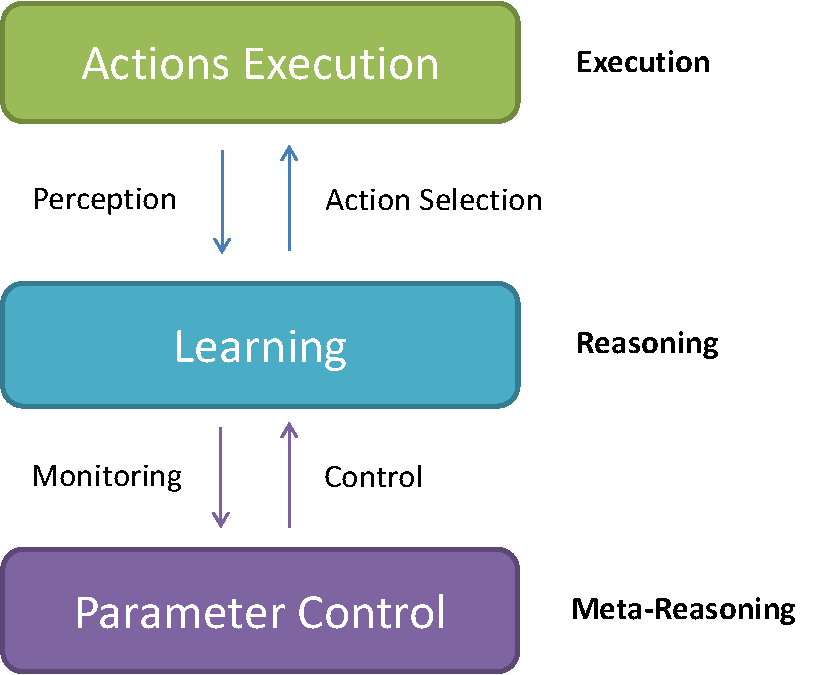
\includegraphics[width=230px]{images/reasoningOnRL}
\caption{Modeling the meta-level reasoning in reinforcement learning.}
\label{fig:reasoningOnRL}
\end{figure}

Our approach to meta-level reasoning consists of varying the learning-rate (known as $\alpha-$value)
to allow an agent to handle dynamic environments. 
More concretely, at the meta-level, we apply RL to learn the $\alpha-$value used as the learning-rate at the object-level RL. 
In other words, we apply reinforcement learning to control the parameters of reinforcement learning. 

The difference between RL applied at the meta-level and RL applied at the object-level is that, at the object-level, we learn Q-value for the action-state pair, increasing it when we have positive feedback and decreasing it when we have negative feedback. 
Conversely, at the meta-level, what we learn in the $\alpha$-value, by decreasing it when we have positive feedback and increasing it when we have negative feedback --- that is, making mistakes means we need to learn at a faster rate. 
Our approach to \textit{meta-level reinforcement learning} is shown in Algorithm~\ref{alg:meta-rl}. 

\begin{algorithm}
	\caption{Meta-Level Reinforcement Learning}
	\label{alg:meta-rl} 
	\begin{algorithmic}[1]
		\REQUIRE $s, a, R$
		\STATE $\alpha \gets \alpha - (0.05 * R)$ \label{meta-rl:line:meta-level}
		\item[]
		\IF{$\alpha < 0$} \label{meta-rl:line:alpha-begin}
			\STATE $\alpha \gets 0$
		\ENDIF
		\IF{$\alpha > 1$}
			\STATE $\alpha \gets 1$
		\ENDIF \label{meta-rl:line:alpha-end}
		\item[]
		\STATE $Q(s,a) \gets Q(s,a) + (\alpha * R)$ \label{meta-rl:line:qlearning}
	\end{algorithmic}
\end{algorithm}

The meta-level reinforcement learning algorithm requires the same parameters as Q-learning:
a state $s$, an action $a$ and a reward $R$.
In Line~\ref{meta-rl:line:meta-level} we apply the RL update rule for the $\alpha$-value used for the object-level Q-learning algorithm. 
At this point, we are learning the learning-rate, and as we saw, $\alpha$ decreases with positive rewards. 
We use a small constant learning-rate of $0.05$ for the meta-level update rule and bound it between $0$ and $1$ (Lines~\ref{meta-rl:line:alpha-begin}--\ref{meta-rl:line:alpha-end}) to ensure it remains a consistent learning-rate value for Q-learning. 
Such a small learning-rate at the meta-level aims to ensure that while we are constantly updating the object-level learning-rate, we avoid high variations. 
Finally, in Line~\ref{meta-rl:line:qlearning} we use the standard update rule for Q-learning,
using the adapted learning-rate. 
As the algorithm is nothing but a sequence of mathematical operations, it is really efficient when it comes to time. 
Thus, it is able to execute in few clock cycles and could be utilized in real-time after each action execution.

Since we are modifying the learning-rate based on the feedback obtained by the agent, and increasing it when the agent detects that its knowledge is no longer up to date, we can also use this value to guide the exploration policy. 
Thus, we also modify the $\epsilon-$greedy action selection algorithm.
Instead of keeping the exploitation-rate ($\epsilon-$value) constant, we apply the same meta-level reasoning to the $\epsilon-$value, increasing the exploration rate, whenever we find that the agent must increase its learning-rate ---  the more the agent wants to learn, the more it wants to explore;
if there is nothing to learn, there is nothing to explore.
To accomplish this, we define the exploitation-rate as been always equal to the learning-rate:
\[
	\epsilon = \alpha
\]



